% =====================================================================
\newpage
\section{Анализ клеточного автомата}
\label{sec:analysis}

Начальные условия всех экспериментов можно воспроизвести в программе: случайные начальные условия задаются плотностью и значением \texttt{seed}, простые паттерны --- ручным вводом.

\subsection{Свойства правила}

Из таблицы истинности (табл.~\ref{tab:truth}) следуют свойства, которые определяют поведение автомата.
\begin{enumerate}
	\item {Пустое поле неподвижно.} Конфигурация $idx = 0$ переходит в 0, поэтому из пустого поля ничего не возникает: $t_0 = 0$, $p = 1$.
	\item {Полностью заполненное поле вымирает за один шаг.} Конфигурация $idx = 31$ переходит в 0, поэтому на следующем шаге все клетки мертвые, далее поле пустое: $t_0 = 1$, $p = 1$.
	\item Правило несимметрично относительно поворотов и отражений. Мертвая клетка рождается только при $idx \in \{2, 6, 7, 10, 15\}$, и во всех этих случаях жив западный сосед ($W = 1$). Значит, рождение возможно только при живом западном соседе: один западный сосед вызывает рождение ($idx = 2 \to 1$), тогда как одиночные северный, восточный или южный соседи --- нет ($idx = 8, 4, 1 \to 0$). В результате у динамики есть выделенное направление --- на восток (вправо).
	\item Если живые клетки находятся только в одной строке, то клетки соседних строк видят лишь одного живого соседа по вертикали ($idx = 1$ или $idx = 8$) и не рождаются. Значит, конфигурация, занимающая одну строку, остается в этой строке. Внутри строки ($N = S = 0$) правило сводится к одномерному элементарному клеточному автомату с окрестностью $(W, C, E)$:
	\[
		C^{t+1} = W^t \oplus (C^t \wedge E^t),
	\]
	что соответствует элементарному правилу 120 по нумерации Вольфрама.
	\item {Пустые строки остаются пустыми.} Западный сосед клетки находится в той же строке, поэтому по свойству 3 в строке без живых клеток ни одна клетка родиться не может. Следовательно, множество строк, содержащих живые клетки, со временем не расширяется, а может только сокращаться: паттерн растет только по горизонтали. Строки при этом не независимы: через соседей $N$ и $S$ они влияют на выживание и рождение клеток друг друга (например, $idx = 10$ и $idx = 15$).
\end{enumerate}

\subsection{Простые паттерны}

\subsubsection*{Одиночная клетка}

Одиночная живая клетка умирает ($idx = 16 \to 0$), а клетка справа от нее рождается, так как видит живого западного соседа ($idx = 2 \to 1$). Остальные соседи живой клетки не рождаются. В результате клетка за каждый шаг сдвигается на одну позицию вправо (рис.~\ref{fig:single}), т.\,е. является простейшим «глайдером», движущимся с максимально возможной для окрестности фон Неймана скоростью. Дойдя до правого края, клетка появляется у левого (тор), поэтому на поле $n \times n$ она возвращается в исходное положение через $n$ шагов: $t_0 = 0$, $p = n$. На рис.~\ref{fig:single} показано поле $7 \times 7$, на котором период равен 7.

\begin{figure}[H]
	\centering
	\begin{minipage}{0.3\textwidth}\centering\console{single_0}\end{minipage}
	\begin{minipage}{0.3\textwidth}\centering\console{single_1}\end{minipage}
	\begin{minipage}{0.3\textwidth}\centering\console{single_2}\end{minipage}\\[3mm]
	\begin{minipage}{0.24\textwidth}\centering\console{single_3}\end{minipage}
	\begin{minipage}{0.24\textwidth}\centering\console{single_4}\end{minipage}
	\begin{minipage}{0.48\textwidth}\centering\console{single_7}\end{minipage}
	\caption{Движение одиночной клетки на поле $7 \times 7$}
	\label{fig:single}
\end{figure}

\subsubsection*{Диагонали}

Диагональ из трех клеток ведет себя по-разному в зависимости от направления. У диагонали «$\backslash$» (сверху слева вниз вправо) за один шаг погибают все три клетки, но рождается одна клетка справа от нижней, так что паттерн сводится к одиночной клетке-глайдеру (рис.~\ref{fig:diagb}): $t_0 = 1$, $p = n$.

\begin{figure}[H]
	\centering
	\begin{minipage}{0.23\textwidth}\centering\console{diagb_0}\end{minipage}
	\begin{minipage}{0.23\textwidth}\centering\console{diagb_1}\end{minipage}
	\begin{minipage}{0.23\textwidth}\centering\console{diagb_2}\end{minipage}
	\begin{minipage}{0.23\textwidth}\centering\console{diagb_3}\end{minipage}
	\caption{Эволюция диагонали «$\backslash$» на поле $9 \times 9$}
	\label{fig:diagb}
\end{figure}

Диагональ «/» (сверху справа вниз влево) сама является глайдером: за каждый шаг она целиком сдвигается на одну клетку вправо, сохраняя форму (рис.~\ref{fig:diagf}), поэтому $t_0 = 0$, $p = n$.

\begin{figure}[H]
	\centering
	\begin{minipage}{0.23\textwidth}\centering\console{diagf_0}\end{minipage}
	\begin{minipage}{0.23\textwidth}\centering\console{diagf_1}\end{minipage}
	\begin{minipage}{0.23\textwidth}\centering\console{diagf_2}\end{minipage}
	\begin{minipage}{0.23\textwidth}\centering\console{diagf_3}\end{minipage}
	\caption{Эволюция диагонали «/» на поле $9 \times 9$}
	\label{fig:diagf}
\end{figure}

\subsubsection*{Горизонтальные паттерны}

Паттерн из живых клеток одной строки, согласно свойству 4, развивается только внутри этой строки по одномерному правилу 120. На рис.~\ref{fig:hpair} показана эволюция пары соседних клеток: в строке возникает нерегулярная последовательность живых клеток, которая смещается вправо. На поле $20 \times 20$ такая эволюция выходит на цикл с периодом 5240 после предпериода 785 шагов (табл.~\ref{tab:patterns}).

\begin{figure}[H]
	\centering
	\begin{minipage}{0.3\textwidth}\centering\console{hpair_0}\end{minipage}
	\begin{minipage}{0.3\textwidth}\centering\console{hpair_1}\end{minipage}
	\begin{minipage}{0.3\textwidth}\centering\console{hpair_2}\end{minipage}\\[3mm]
	\begin{minipage}{0.3\textwidth}\centering\console{hpair_3}\end{minipage}
	\begin{minipage}{0.3\textwidth}\centering\console{hpair_4}\end{minipage}
	\caption{Эволюция горизонтальной пары клеток на поле $11 \times 11$}
	\label{fig:hpair}
\end{figure}

\subsubsection*{Двумерные паттерны}

Если живые клетки находятся в нескольких строках, то строки влияют друг на друга через северного и южного соседей, и эволюция уже не сводится к одномерному правилу. Однако по свойству 5 паттерн никогда не выходит за пределы строк, в которых он был задан. На рис.~\ref{fig:vpair} и~\ref{fig:cross} показаны первые шаги эволюции вертикальной пары клеток и «креста»: в обоих случаях паттерн разрастается по горизонтали внутри своих строк и одновременно смещается вправо.

\begin{figure}[H]
	\centering
	\begin{minipage}{0.23\textwidth}\centering\console{vpair_0}\end{minipage}
	\begin{minipage}{0.23\textwidth}\centering\console{vpair_1}\end{minipage}
	\begin{minipage}{0.23\textwidth}\centering\console{vpair_2}\end{minipage}
	\begin{minipage}{0.23\textwidth}\centering\console{vpair_3}\end{minipage}
	\caption{Эволюция вертикальной пары клеток на поле $9 \times 9$}
	\label{fig:vpair}
\end{figure}

\begin{figure}[H]
	\centering
	\begin{minipage}{0.23\textwidth}\centering\console{cross_0}\end{minipage}
	\begin{minipage}{0.23\textwidth}\centering\console{cross_1}\end{minipage}
	\begin{minipage}{0.23\textwidth}\centering\console{cross_2}\end{minipage}
	\begin{minipage}{0.23\textwidth}\centering\console{cross_3}\end{minipage}
	\caption{Эволюция паттерна «крест» на поле $9 \times 9$}
	\label{fig:cross}
\end{figure}

Вертикальная пара за один шаг превращается в квадрат $2 \times 2$ (рис.~\ref{fig:vpair}, поколение 1), поэтому дальше эти паттерны эволюционируют одинаково, а их предпериоды в таблице~\ref{tab:patterns} отличаются на 1. Сам квадрат $2 \times 2$ показан на рис.~\ref{fig:square}: верхняя строка вытягивается вправо, нижняя теряет левые клетки.

\begin{figure}[H]
	\centering
	\begin{minipage}{0.23\textwidth}\centering\console{square_0}\end{minipage}
	\begin{minipage}{0.23\textwidth}\centering\console{square_1}\end{minipage}
	\begin{minipage}{0.23\textwidth}\centering\console{square_2}\end{minipage}
	\begin{minipage}{0.23\textwidth}\centering\console{square_3}\end{minipage}
	\caption{Эволюция квадрата $2 \times 2$ на поле $9 \times 9$}
	\label{fig:square}
\end{figure}

На рис.~\ref{fig:lshape}--\ref{fig:square3} показаны паттерны, занимающие три строки: буква «L», вертикальная линия и квадрат $3 \times 3$. Средняя строка «L» с одной клеткой сразу погибает и по свойству 5 остается пустой, поэтому верхняя и нижняя строки дальше развиваются независимо, каждая по одномерному правилу 120 (свойство 4); этим объясняется совпадение периода «L» с периодом горизонтальных паттернов (табл.~\ref{tab:patterns}). У вертикальной линии и квадрата $3 \times 3$ все три строки сохраняют живые клетки, и паттерн растет вправо, оставаясь в своих трех строках.

\begin{figure}[H]
	\centering
	\begin{minipage}{0.23\textwidth}\centering\console{lshape_0}\end{minipage}
	\begin{minipage}{0.23\textwidth}\centering\console{lshape_1}\end{minipage}
	\begin{minipage}{0.23\textwidth}\centering\console{lshape_2}\end{minipage}
	\begin{minipage}{0.23\textwidth}\centering\console{lshape_3}\end{minipage}
	\caption{Эволюция паттерна «L» на поле $9 \times 9$}
	\label{fig:lshape}
\end{figure}

\begin{figure}[H]
	\centering
	\begin{minipage}{0.23\textwidth}\centering\console{vline_0}\end{minipage}
	\begin{minipage}{0.23\textwidth}\centering\console{vline_1}\end{minipage}
	\begin{minipage}{0.23\textwidth}\centering\console{vline_2}\end{minipage}
	\begin{minipage}{0.23\textwidth}\centering\console{vline_3}\end{minipage}
	\caption{Эволюция вертикальной линии из 3 клеток на поле $9 \times 9$}
	\label{fig:vline}
\end{figure}

\begin{figure}[H]
	\centering
	\begin{minipage}{0.23\textwidth}\centering\console{square3_0}\end{minipage}
	\begin{minipage}{0.23\textwidth}\centering\console{square3_1}\end{minipage}
	\begin{minipage}{0.23\textwidth}\centering\console{square3_2}\end{minipage}
	\begin{minipage}{0.23\textwidth}\centering\console{square3_3}\end{minipage}
	\caption{Эволюция квадрата $3 \times 3$ на поле $9 \times 9$}
	\label{fig:square3}
\end{figure}

Результаты запуска автомата на простых паттернах, помещенных в центр поля $20 \times 20$, приведены в таблице~\ref{tab:patterns}.

\begin{table}[H]
	\centering
	\caption{Простые паттерны на поле $20 \times 20$}
	\label{tab:patterns}
	\begin{tabular}{|l|c|c|c|}
		\hline
		Паттерн & Предпериод $t_0$ & Период $p$ & Живых$^*$ \\
		\hline
		одна клетка & 0 & 20 & 1 \\
		диагональ из 3 клеток «$\backslash$» & 1 & 20 & 1 \\
		диагональ из 3 клеток «/» & 0 & 20 & 3 \\
		крест & 11 & 40 & 9 \\
		две клетки по горизонтали & 785 & 5240 & 10 \\
		горизонтальная линия из 3 клеток & 784 & 5240 & 10 \\
		две клетки по вертикали & 428 & 21240 & 13 \\
		квадрат $2 \times 2$ & 427 & 21240 & 13 \\
		квадрат $3 \times 3$ & 1036 & 5240 & 21 \\
		буква «L» & 786 & 5240 & 20 \\
		вертикальная линия из 3 клеток & \multicolumn{2}{c|}{не найден за $10^5$ шагов} & 15 \\
		\hline
	\end{tabular}

	\smallskip
	% \footnotesize $^*$ Число живых клеток в момент обнаружения цикла ($t = t_0 + p$), для вертикальной линии --- после $10^5$ шагов.
\end{table}

Видно, что даже паттерны из 2--5 клеток в большинстве случаев проходят длинный переходный процесс (сотни шагов) и выходят на циклы длиной в тысячи шагов. Исключения --- паттерны, которые за несколько шагов сводятся к одиночной движущейся клетке (диагональ «$\backslash$») или к небольшой движущейся структуре (крест), а также диагональ «/», которая сама является глайдером.

\subsection{Случайные начальные условия}

На рис.~\ref{fig:random} показана эволюция случайной начальной конфигурации на поле $30 \times 30$ с плотностью живых клеток 30\,\% (\texttt{seed} = 1). Уже через несколько шагов поле перестает напоминать начальную конфигурацию, и далее картина остается неупорядоченной: устойчивых или периодических локальных структур не возникает, характерны короткие горизонтальные цепочки живых клеток, движущиеся вправо.

\begin{figure}[H]
	\centering
	\begin{minipage}{0.48\textwidth}\centering\console[\consoletiny]{random_0}\end{minipage}\hfill
	\begin{minipage}{0.48\textwidth}\centering\console[\consoletiny]{random_1}\end{minipage}\\[2mm]
	\begin{minipage}{0.48\textwidth}\centering\console[\consoletiny]{random_10}\end{minipage}\hfill
	\begin{minipage}{0.48\textwidth}\centering\console[\consoletiny]{random_100}\end{minipage}\\[2mm]
	\begin{minipage}{0.48\textwidth}\centering\console[\consoletiny]{random_1000}\end{minipage}
	\caption{Эволюция случайной конфигурации на поле $30 \times 30$ (плотность 30\,\%, seed = 1)}
	\label{fig:random}
\end{figure}

Для оценки того, как меняется число живых клеток, были проведены эксперименты на поле $50 \times 50$: для каждой начальной плотности (10, 30, 50, 70 и 90\,\%) выполнено 20 запусков ($\text{seed} = 1..20$) по 100 поколений, затем доля живых клеток усреднена по запускам (рис.~\ref{fig:population}). Независимо от начальной плотности доля живых клеток быстро (за 5--10 поколений) смещается к значениям около 0,1--0,25: при плотностях 50, 70 и 90\,\% она резко падает, при 10\,\% немного возрастает. К 100-му поколению доли для плотностей 30, 50 и 70\,\% сближаются (0,204; 0,208; 0,202), а для плотностей 10 и 90\,\% продолжают медленно сходиться к тому же уровню (0,161 и 0,149).

\begin{figure}[H]
	\centering
	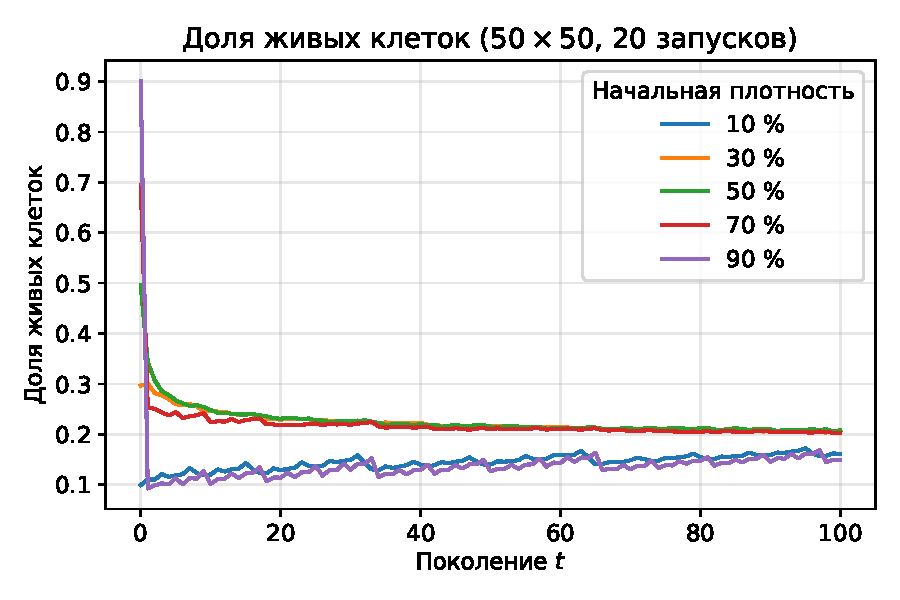
\includegraphics[width=1\textwidth]{automaton_analysis.pdf}
	\caption{Доля живых клеток в зависимости от номера поколения (поле $50 \times 50$, среднее по 20 запускам)}
	\label{fig:population}
\end{figure}

\subsection{Периодичность}

В таблице~\ref{tab:periods} приведены предпериоды и периоды, найденные программой для полей $n \times n$ при $n = 3..16$, плотности 50\,\% и \texttt{seed} = 1..10 (ограничение --- $10^5$ шагов, как в программе).

\begin{table}[H]
	\centering
	\caption{Предпериоды и периоды для случайных конфигураций (плотность 50\,\%, 10 запусков)}
	\label{tab:periods}
	\begin{tabular}{|c|c|c|l|c|}
		\hline
		$n$ & $2^{n^2}$ & $t_0$ (мин--макс) & Найденные периоды $p$ & Не найден \\
		\hline
		3  & $5{,}1 \cdot 10^{2}$  & 0--5     & 1, 3                  & 0 \\
		4  & $6{,}6 \cdot 10^{4}$  & 1--14    & 2, 4, 18              & 0 \\
		5  & $3{,}4 \cdot 10^{7}$  & 1--12    & 5, 15, 45             & 0 \\
		6  & $6{,}9 \cdot 10^{10}$ & 8--24    & 1, 3, 6               & 0 \\
		7  & $5{,}6 \cdot 10^{14}$ & 2--46    & 7, 28, 49, 196        & 0 \\
		8  & $1{,}8 \cdot 10^{19}$ & 10--57   & 30, 36, 120, 180, 360 & 0 \\
		9  & $2{,}4 \cdot 10^{24}$ & 30--154  & 9, 36, 54, 108        & 0 \\
		10 & $1{,}3 \cdot 10^{30}$ & 30--118  & 205, 410, 1640        & 0 \\
		11 & $2{,}7 \cdot 10^{36}$ & 47--139  & 176, 1232             & 0 \\
		12 & $2{,}2 \cdot 10^{43}$ & 50--311  & 1, 12, 24, 168        & 0 \\
		13 & $7{,}5 \cdot 10^{50}$ & 125--190 & 416, 4576, 12896, 22880 & 5 \\
		14 & $1{,}0 \cdot 10^{59}$ & 179--427 & 15680, 28224          & 2 \\
		15 & $5{,}4 \cdot 10^{67}$ & 134--289 & 450, 32850, 59850     & 7 \\
		16 & $1{,}2 \cdot 10^{77}$ & 189--745 & 2688, 13440           & 0 \\
		\hline
	\end{tabular}
\end{table}

На полях $n = 17, 18$ циклы еще находятся (например, $t_0 = 746$, $p = 2533$ при $n = 17$; $t_0 = 554$, $p = 23\,976$ при $n = 18$), но уже при $n = 20$ и $n = 25$ ни в одном из запусков цикл за $10^5$ шагов не обнаружен; при $n = 30$ (плотность 30\,\%) цикл не найден за $10^5$ шагов.


Из таблицы видно, что
\begin{itemize}
	\item при $n \ge 10$ предпериод невелик по сравнению с периодом, на малых полях, наоборот, переходный процесс может быть длиннее короткого цикла (например, при $n = 6$: $t_0 = 8..24$, $p = 1..6$);
	\item период в целом быстро растет с размером поля (от единиц и десятков при $n \le 6$ до десятков тысяч при $n \ge 13$), хотя рост неравномерен и зависит от арифметических свойств $n$;
	\item периоды часто кратны $n$, что связано со сдвигом структур вправо: конфигурация возвращается в исходное положение после целого числа оборотов вокруг тора;
	\item найденные периоды несравнимо меньше числа $2^{n^2}$ возможных конфигураций, однако при $n \ge 20$ они уже недоступны для прямого перебора.
\end{itemize}

\subsection{Классификация по Вольфраму}

По результатам анализа автомат с правилом 20\,874\,436 (порядок $C$, $N$, $E$, $W$, $S$) относится к {классу III} (хаотическое поведение):
\begin{itemize}
	\item эволюция случайных конфигураций не приводит ни к однородному состоянию (класс I), ни к набору простых устойчивых или периодических структур (класс II): поле остается неупорядоченным;
	\item длины циклов на торе быстро растут с размером поля и уже при $n \ge 20$ не наблюдаются за $10^5$ шагов;
	\item даже простые паттерны из нескольких клеток порождают длительную нерегулярную эволюцию.
\end{itemize}

У автомата есть и черты других классов: на малых полях ($n \le 6$) встречаются неподвижные точки и короткие циклы, а одиночная клетка и диагональ из трех клеток «/» являются движущимися локализованными структурами («глайдерами»). Однако на случайных начальных конфигурациях такие структуры не сохраняются и растворяются в хаотическом фоне, поэтому отнести автомат к IV классу нельзя.
